\documentclass[10pt, landscape, twocolumn]{article}

\usepackage[margin=0.5in, columnsep=0.4in]{geometry}
\usepackage{amsmath, amssymb, amsthm}
\usepackage{xcolor}
\usepackage{tabularx}
\usepackage{tikz}
\usetikzlibrary{arrows.meta, positioning, calc, shapes.geometric, 3d}
\usepackage{enumitem}
\usepackage{mathpazo}
\usepackage{booktabs}
\usepackage{multicol}

\pagestyle{empty}
\setlength{\parindent}{0pt}
\setlength{\parskip}{4pt}

\AtBeginDocument{
  \setlength{\abovedisplayskip}{4pt}
  \setlength{\belowdisplayskip}{4pt}
  \setlength{\abovedisplayshortskip}{2pt}
  \setlength{\belowdisplayshortskip}{2pt}
}

\definecolor{themeblue}{RGB}{0, 90, 160}
\definecolor{themegray}{RGB}{80, 80, 80}

\newcommand{\cheatsheetsection}[1]{
    \vspace{0.8em}
    {\color{themeblue}\large\bfseries #1} \par
    \vspace{-0.4em}
    {\color{themeblue}\rule{\linewidth}{1pt}} \par
    \vspace{0.3em}
}

\newcommand{\cheatsheetsubsection}[1]{
    \vspace{0.5em}
    {\color{themeblue}\normalsize\bfseries #1} \par
    \vspace{0.2em}
}

\begin{document}

\begin{center}
    \vspace{-1em}
    {\color{themeblue}\huge\bfseries Vector Calculus Cheat Sheet}\\[0.1em]
    {\color{themegray}\small Comprehensive Reference for Engineering, Physics, and Differential Geometry}\\[0.4em]
    {\color{themegray}\footnotesize \textbf{By Roberto León Landeros}}
\end{center}
\vspace{-1em}

\cheatsheetsection{1. Index Notation \& Tensor Algebra}

\cheatsheetsubsection{Einstein Summation Convention}
Repeated indices within a term imply summation over that index: $a_i b_i = \sum_{i=1}^3 a_i b_i$. A free index appears once per term.

\cheatsheetsubsection{Kronecker Delta ($\delta_{ij}$)}
Acts as an identity matrix and an index filter: $\delta_{ij} A_j = A_i$. In $\mathbb{R}^3$, $\delta_{ii} = 3$.
\[
\delta_{ij} = \begin{cases} 
1 & \text{if } i = j \\ 
0 & \text{if } i \neq j 
\end{cases}
\]

\cheatsheetsubsection{Levi-Civita Symbol ($\epsilon_{ijk}$)}
\[
\epsilon_{ijk} = \begin{cases} 
+1 & \text{even permutation of } (1,2,3) \\ 
-1 & \text{odd permutation of } (1,2,3) \\ 
0 & \text{any repeated index} 
\end{cases}
\]
Cross product definition: $(\mathbf{A} \times \mathbf{B})_i = \epsilon_{ijk} A_j B_k$. \\
Scalar triple product: $\mathbf{A} \cdot (\mathbf{B} \times \mathbf{C}) = \epsilon_{ijk} A_i B_j C_k$.

\cheatsheetsubsection{Tensor Identities \& Symmetry}
\begin{itemize}[leftmargin=*, nosep]
    \item \textbf{Epsilon-Delta Identity:} $\epsilon_{ijk}\epsilon_{imn} = \delta_{jm}\delta_{kn} - \delta_{jn}\delta_{km}$.
    \item \textbf{Contractions:} $\epsilon_{ijk}\epsilon_{ijn} = 2\delta_{kn}$, and $\epsilon_{ijk}\epsilon_{ijk} = 6$.
    \item \textbf{Cross Product Matrix:} $\mathbf{A} \times \mathbf{B} = [\mathbf{A}]_\times \mathbf{B}$, where $[\mathbf{A}]_\times$ is the skew-symmetric matrix of $\mathbf{A}$.
    \item \textbf{Symmetry Annihilation:} The double dot product of a symmetric tensor $S_{ij} = S_{ji}$ and a skew-symmetric tensor $A_{ij} = -A_{ji}$ is strictly zero: $S_{ij}A_{ij} = 0$.
\end{itemize}

\cheatsheetsection{2. Vector Algebra in $\mathbb{R}^3$}

\cheatsheetsubsection{Dot and Cross Products}
\begin{itemize}[leftmargin=*, nosep]
    \item \textbf{Dot Product:} $\mathbf{u} \cdot \mathbf{v} = |\mathbf{u}||\mathbf{v}|\cos\theta = u_i v_i$. Measures parallel projection. $\mathbf{u} \cdot \mathbf{v} = 0 \implies \mathbf{u} \perp \mathbf{v}$.
    \item \textbf{Cross Product:} $\mathbf{u} \times \mathbf{v} = \mathbf{n} |\mathbf{u}||\mathbf{v}|\sin\theta = \begin{vmatrix} \hat{i} & \hat{j} & \hat{k} \\ u_x & u_y & u_z \\ v_x & v_y & v_z \end{vmatrix}$. Result is orthogonal to $\mathbf{u}$ and $\mathbf{v}$. Magnitude is parallelogram area.
\end{itemize}

\begin{center}
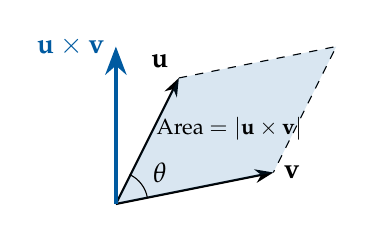
\begin{tikzpicture}[scale=0.8, >=Stealth]
    \draw[->, thick] (0,0) -- (2.5,0.5) node[right] {$\mathbf{v}$};
    \draw[->, thick] (0,0) -- (1,2) node[above left] {$\mathbf{u}$};
    \draw[dashed] (1,2) -- (3.5,2.5) -- (2.5,0.5);
    \fill[themeblue, opacity=0.15] (0,0) -- (2.5,0.5) -- (3.5,2.5) -- (1,2) -- cycle;
    \draw[->, themeblue, ultra thick] (0,0) -- (0,2.5) node[left] {$\mathbf{u} \times \mathbf{v}$};
    \draw (0.5,0.1) arc (10:65:0.5);
    \node at (0.7,0.5) {$\theta$};
    \node at (1.8,1.2) {\footnotesize Area $= |\mathbf{u} \times \mathbf{v}|$};
\end{tikzpicture}
\end{center}

\cheatsheetsubsection{Triple and Quadruple Products}
\textbf{Scalar Triple:} $[\mathbf{u}, \mathbf{v}, \mathbf{w}] = \mathbf{u} \cdot (\mathbf{v} \times \mathbf{w}) = \begin{vmatrix} u_x & u_y & u_z \\ v_x & v_y & v_z \\ w_x & w_y & w_z \end{vmatrix}$. Oriented volume of parallelepiped. Cyclically invariant: $[\mathbf{u}, \mathbf{v}, \mathbf{w}] = [\mathbf{v}, \mathbf{w}, \mathbf{u}]$.

\begin{center}
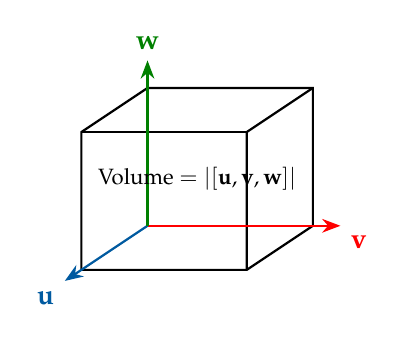
\begin{tikzpicture}[scale=0.7, >=Stealth, x={(-0.6cm,-0.4cm)}, y={(1cm,0cm)}, z={(0cm,1cm)}]
  \coordinate (O) at (0,0,0);
  \coordinate (A) at (2,0,0);
  \coordinate (B) at (0,3,0);
  \coordinate (C) at (0,0,2.5);
  \coordinate (A1) at (2,3,0);
  \coordinate (B1) at (0,3,2.5);
  \coordinate (C1) at (2,0,2.5);
  \coordinate (D) at (2,3,2.5);
  
  \draw[dashed, themegray] (O) -- (A);
  \draw[dashed, themegray] (O) -- (B);
  \draw[dashed, themegray] (O) -- (C);
  
  \draw[thick] (A) -- (A1) -- (B) -- (B1) -- (C) -- (C1) -- cycle;
  \draw[thick] (A1) -- (D) -- (B1);
  \draw[thick] (C1) -- (D);
  
  \draw[->, thick, themeblue] (O) -- (2.5,0,0) node[anchor=north east] {$\mathbf{u}$};
  \draw[->, thick, red] (O) -- (0,3.5,0) node[anchor=north west] {$\mathbf{v}$};
  \draw[->, thick, green!50!black] (O) -- (0,0,3) node[anchor=south] {$\mathbf{w}$};
  
  \node at (1,1.5,1.25) {\footnotesize Volume $= |[\mathbf{u}, \mathbf{v}, \mathbf{w}]|$};
\end{tikzpicture}
\end{center}

\begin{itemize}[leftmargin=*, nosep]
    \item \textbf{Vector Triple:} $\mathbf{A} \times (\mathbf{B} \times \mathbf{C}) = \mathbf{B}(\mathbf{A} \cdot \mathbf{C}) - \mathbf{C}(\mathbf{A} \cdot \mathbf{B})$ (BAC-CAB rule).
    \item \textbf{Jacobi Identity:} $\mathbf{A} \times (\mathbf{B} \times \mathbf{C}) + \mathbf{B} \times (\mathbf{C} \times \mathbf{A}) + \mathbf{C} \times (\mathbf{A} \times \mathbf{B}) = \mathbf{0}$.
    \item \textbf{Lagrange's Identity:} $|\mathbf{A} \times \mathbf{B}|^2 = |\mathbf{A}|^2|\mathbf{B}|^2 - (\mathbf{A} \cdot \mathbf{B})^2$.
    \item \textbf{Scalar Quadruple:} $(\mathbf{A} \times \mathbf{B}) \cdot (\mathbf{C} \times \mathbf{D}) = (\mathbf{A} \cdot \mathbf{C})(\mathbf{B} \cdot \mathbf{D}) - (\mathbf{A} \cdot \mathbf{D})(\mathbf{B} \cdot \mathbf{C})$.
\end{itemize}

\cheatsheetsubsection{Analytic Geometry: Lines, Planes, Surfaces}
\begin{itemize}[leftmargin=*, nosep]
    \item \textbf{Line (Parametric):} $\mathbf{r}(t) = \mathbf{r}_0 + t\mathbf{v}$.
    \item \textbf{Line (Symmetric):} $\frac{x-x_0}{v_x} = \frac{y-y_0}{v_y} = \frac{z-z_0}{v_z}$.
    \item \textbf{Plane (Normal form):} $\mathbf{n} \cdot (\mathbf{r} - \mathbf{r}_0) = 0 \implies a(x-x_0) + b(y-y_0) + c(z-z_0) = 0$.
    \item \textbf{Distance Point $P$ to Plane:} $D = \frac{|ax_p + by_p + cz_p - d|}{\sqrt{a^2+b^2+c^2}}$.
\end{itemize}
\textbf{Quadric Surfaces Base Forms:}\\
Ellipsoid: $\frac{x^2}{a^2} + \frac{y^2}{b^2} + \frac{z^2}{c^2} = 1$. Paraboloid: $z = \frac{x^2}{a^2} + \frac{y^2}{b^2}$.\\
Hyperboloid (1 sheet): $\frac{x^2}{a^2} + \frac{y^2}{b^2} - \frac{z^2}{c^2} = 1$. Cone: $z^2 = \frac{x^2}{a^2} + \frac{y^2}{b^2}$.

\cheatsheetsection{3. Differential Geometry}

\cheatsheetsubsection{Curves and the Frenet-Serret Frame}
\begin{itemize}[leftmargin=*, nosep]
    \item \textbf{Arc Length:} $s(t) = \int_{t_0}^t |\mathbf{r}'(u)| du \implies ds = |\mathbf{r}'(t)|dt$.
    \item \textbf{Tangent:} $\mathbf{T} = \frac{\mathbf{r}'}{|\mathbf{r}'|}$. \quad \textbf{Normal:} $\mathbf{N} = \frac{\mathbf{T}'}{|\mathbf{T}'|}$. \quad \textbf{Binormal:} $\mathbf{B} = \mathbf{T} \times \mathbf{N}$.
    \item \textbf{Curvature ($\kappa$):} Measures deviation from a line. \\ $\kappa = \frac{|\mathbf{T}'|}{|\mathbf{r}'|} = \frac{|\mathbf{r}' \times \mathbf{r}''|}{|\mathbf{r}'|^3}$. Radius of curvature: $R = \frac{1}{\kappa}$.
    \item \textbf{Osculating Circle:} Center of curvature at $\mathbf{c} = \mathbf{r}(s) + \frac{1}{\kappa}\mathbf{N}$.
    \item \textbf{Torsion ($\tau$):} Measures deviation from the osculating plane.
\end{itemize}
\[
\tau = \frac{(\mathbf{r}' \times \mathbf{r}'') \cdot \mathbf{r}'''}{|\mathbf{r}' \times \mathbf{r}''|^2}
\]

\textbf{Frenet-Serret Formulas:}
\begin{equation*}
\begin{bmatrix} \mathbf{T}' \\ \mathbf{N}' \\ \mathbf{B}' \end{bmatrix} = |\mathbf{r}'| \begin{bmatrix} 0 & \kappa & 0 \\ -\kappa & 0 & \tau \\ 0 & -\tau & 0 \end{bmatrix} \begin{bmatrix} \mathbf{T} \\ \mathbf{N} \\ \mathbf{B} \end{bmatrix}
\end{equation*}

\begin{center}
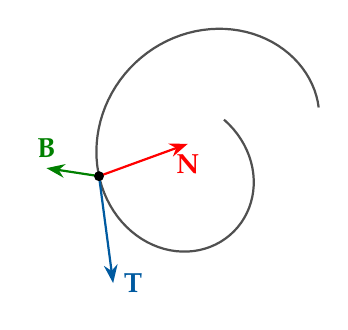
\begin{tikzpicture}[scale=1.2, >=Stealth]
    \draw[thick, themegray, domain=0:4, samples=100] plot ({cos(\x*100)}, {sin(\x*100)}, {\x*0.5});
    \coordinate (P) at ({cos(200)}, {sin(200)}, {2*0.5});
    \draw[->, themeblue, thick] (P) -- ++({-sin(200)}, {cos(200)}, 0.5) node[right] {$\mathbf{T}$};
    \draw[->, red, thick] (P) -- ++({-cos(200)}, {-sin(200)}, 0) node[below] {$\mathbf{N}$};
    \draw[->, green!50!black, thick] (P) -- ++({sin(200)*0.5}, {-cos(200)*0.5}, 1) node[above] {$\mathbf{B}$};
    \fill (P) circle (1.5pt);
\end{tikzpicture}
\end{center}

\vspace{-2}
\cheatsheetsubsection{Surface Geometry Fundamentals}
For a parametrized surface $\mathbf{r}(u,v)$:
\begin{itemize}[leftmargin=*, nosep]
    \item \textbf{Normal Vector:} $\mathbf{n} = \frac{\mathbf{r}_u \times \mathbf{r}_v}{|\mathbf{r}_u \times \mathbf{r}_v|}$.
    \item \textbf{First Fundamental Form (Metric):} $I = E\,du^2 + 2F\,du\,dv + G\,dv^2$. \\
    $E = \mathbf{r}_u \cdot \mathbf{r}_u$, $F = \mathbf{r}_u \cdot \mathbf{r}_v$, $G = \mathbf{r}_v \cdot \mathbf{r}_v$. \\
    Area element: $dS = \sqrt{EG - F^2} \, du \, dv = |\mathbf{r}_u \times \mathbf{r}_v| \, du \, dv$.
    \item \textbf{Second Fundamental Form:} $II = L\,du^2 + 2M\,du\,dv + N\,dv^2$. \\
    $L = \mathbf{r}_{uu} \cdot \mathbf{n}$, $M = \mathbf{r}_{uv} \cdot \mathbf{n}$, $N = \mathbf{r}_{vv} \cdot \mathbf{n}$.
    \item \textbf{Gaussian Curvature:} $K = \frac{LN - M^2}{EG - F^2}$. 
    \item \textbf{Gauss's Theorema Egregium:} Gaussian curvature $K$ is an intrinsic property; it remains invariant under local isometries (bending without stretching).
    \item \textbf{Mean Curvature:} $H = \frac{EN + GL - 2FM}{2(EG - F^2)}$.
    \item \textbf{Geodesics:} Curves of shortest path on a surface where the acceleration is strictly normal to the surface: $\mathbf{r}'' \times \mathbf{n} = \mathbf{0}$.
\end{itemize}

\cheatsheetsection{4. Coordinate Systems \& Transformations}

\cheatsheetsubsection{General Orthogonal Curvilinear Coordinates}
Coordinates $(q_1, q_2, q_3)$. Position vector $\mathbf{r}(q_1, q_2, q_3)$.
\begin{itemize}[leftmargin=*, nosep]
    \item \textbf{Scale Factors:} $h_i = \left| \frac{\partial \mathbf{r}}{\partial q_i} \right|$. Metric: $ds^2 = h_1^2 dq_1^2 + h_2^2 dq_2^2 + h_3^2 dq_3^2$.
    \item \textbf{Volume element:} $dV = h_1 h_2 h_3 \, dq_1 \, dq_2 \, dq_3$.
    \item \textbf{Jacobian Matrix ($J$):} $J_{ij} = \frac{\partial x_i}{\partial q_j}$. $dV = |\det(J)| \, dq_1 \, dq_2 \, dq_3$.
\end{itemize}

\cheatsheetsubsection{Cylindrical Coordinates $(\rho, \phi, z)$}
$x = \rho \cos \phi, \quad y = \rho \sin \phi, \quad z = z$. \\
$h_\rho = 1, \quad h_\phi = \rho, \quad h_z = 1 \implies dV = \rho \, d\rho \, d\phi \, dz$. \\
\textbf{Unit Vector Derivatives:} $\frac{\partial \hat{\rho}}{\partial \phi} = \hat{\phi}, \quad \frac{\partial \hat{\phi}}{\partial \phi} = -\hat{\rho}$.

\vspace{-0.4em}
{\centering
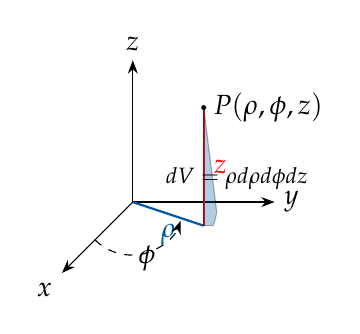
\begin{tikzpicture}[scale=0.6, >=Stealth]
  \draw[->] (0,0) -- (3,0) node[right] {$y$};
  \draw[->] (0,0) -- (-1.5,-1.5) node[below left] {$x$};
  \draw[->] (0,0) -- (0,3) node[above] {$z$};
  \draw[thick, themeblue] (0,0) -- (1.5,-0.5) node[midway, below] {$\rho$};
  \draw[thick, red] (1.5,-0.5) -- (1.5, 2) node[midway, right] {$z$};
  \draw[->, dashed] (-0.8,-0.8) arc (225:340:1.1);
  \node at (0.3,-1.2) {$\phi$};
  \fill (1.5,2) circle (1.5pt) node[right] {$P(\rho, \phi, z)$};
  
  \draw[fill=themeblue, opacity=0.3] (1.5, -0.5) -- (1.7, -0.5) arc (340:350:1.7) -- (1.5, 2) -- cycle;
  \node at (2.2, 0.5) {\footnotesize $dV = \rho d\rho d\phi dz$};
\end{tikzpicture}\par}
\vspace{-0.4em}

\textbf{Unit Vector Transformation Matrix (Cartesian to Cylindrical):}
\vspace{0.2em}
{\centering
$ \begin{bmatrix} \hat{\rho} \\ \hat{\phi} \\ \hat{z} \end{bmatrix} = \begin{bmatrix} \cos\phi & \sin\phi & 0 \\ -\sin\phi & \cos\phi & 0 \\ 0 & 0 & 1 \end{bmatrix} \begin{bmatrix} \hat{i} \\ \hat{j} \\ \hat{k} \end{bmatrix} $\par}
\vspace{0.6em}

\cheatsheetsubsection{Spherical Coordinates $(r, \theta, \phi)$}
Physics Convention: $\theta$ is polar (colatitude), $\phi$ is azimuthal (longitude). \\
$x = r \sin\theta \cos\phi, \quad y = r \sin\theta \sin\phi, \quad z = r \cos\theta$. \\
$h_r = 1, \quad h_\theta = r, \quad h_\phi = r\sin\theta \implies dV = r^2\sin\theta \, dr \, d\theta \, d\phi$.

\vspace{-0.4em}
{\centering
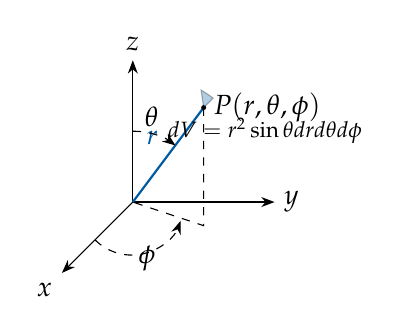
\begin{tikzpicture}[scale=0.6, >=Stealth]
  \draw[->] (0,0) -- (3,0) node[right] {$y$};
  \draw[->] (0,0) -- (-1.5,-1.5) node[below left] {$x$};
  \draw[->] (0,0) -- (0,3) node[above] {$z$};
  \draw[thick, themeblue] (0,0) -- (1.5, 2) node[midway, above left] {$r$};
  \draw[dashed] (1.5, 2) -- (1.5, -0.5) -- (0,0);
  \draw[->, dashed] (0, 1.5) arc (90:53:1.5);
  \node at (0.4, 1.8) {$\theta$};
  \draw[->, dashed] (-0.8,-0.8) arc (225:340:1.1);
  \node at (0.3,-1.2) {$\phi$};
  \fill (1.5,2) circle (1.5pt) node[right] {$P(r, \theta, \phi)$};
  
  \draw[fill=themeblue, opacity=0.3] (1.5, 2) -- (1.7, 2.2) arc (53:60:2.5) -- (1.5, 2) -- cycle;
  \node at (2.8, 1.5) {\footnotesize $dV = r^2\sin\theta dr d\theta d\phi$};
\end{tikzpicture}\par}
\newpage
\textbf{Unit Vector Transformation Matrix (Cartesian to Spherical):}
\vspace{0.2em}
{\centering
$ \begin{bmatrix} \hat{r} \\ \hat{\theta} \\ \hat{\phi} \end{bmatrix} = \begin{bmatrix} \sin\theta\cos\phi & \sin\theta\sin\phi & \cos\theta \\ \cos\theta\cos\phi & \cos\theta\sin\phi & -\sin\theta \\ -\sin\phi & \cos\phi & 0 \end{bmatrix} \begin{bmatrix} \hat{i} \\ \hat{j} \\ \hat{k} \end{bmatrix} $\par}
\vspace{0.2em}\
{\footnotesize \textbf{Note:} To convert Spherical to Cartesian, use the transpose of the matrix above since it is orthogonal ($Q^{-1} = Q^T$).}

\cheatsheetsection{5. Differential Calculus \& Optimization}

\cheatsheetsubsection{Linear Approximation \& Tangent Planes}
\textbf{Total Differential:} $df = \frac{\partial f}{\partial x} dx + \frac{\partial f}{\partial y} dy + \frac{\partial f}{\partial z} dz = \nabla f \cdot d\mathbf{r}$. \\
\textbf{Tangent Plane to $F(x,y,z)=c$:} $\nabla F(x_0, y_0, z_0) \cdot \langle x-x_0, y-y_0, z-z_0 \rangle = 0$. \\
\textbf{Taylor Series (2nd Order):} $f(x,y) \approx f(a,b) + f_x(x-a) + f_y(y-b) + \frac{1}{2!}\left[ f_{xx}(x-a)^2 + 2f_{xy}(x-a)(y-b) + f_{yy}(y-b)^2 \right]$.

\cheatsheetsubsection{Directional Derivative \& Triple Product Rule}
\textbf{Directional Derivative:} $D_{\mathbf{u}}f = \nabla f \cdot \mathbf{u}$. Rate of change in direction of unit vector $\mathbf{u}$. Max rate of change is $|\nabla f|$. \\
\textbf{Triple Product Rule (Thermodynamics):} If $F(x,y,z)=0$, then $\left(\frac{\partial x}{\partial y}\right)_z \left(\frac{\partial y}{\partial z}\right)_x \left(\frac{\partial z}{\partial x}\right)_y = -1$.

\cheatsheetsubsection{Optimization: Hessian \& Lagrange}
\textbf{Hessian Matrix ($H$):} $H_{ij} = \frac{\partial^2 f}{\partial x_i \partial x_j}$. \\
For $f(x,y)$, Discriminant $D = \det(H) = f_{xx}f_{yy} - (f_{xy})^2$. \\
$D>0, f_{xx}>0 \implies$ Min. \quad $D>0, f_{xx}<0 \implies$ Max. \quad $D<0 \implies$ Saddle. \\
\textbf{Lagrange Multipliers:} Optimize $f(\mathbf{r})$ subject to constraint $g(\mathbf{r})=k$: $\nabla f = \lambda \nabla g$. For two constraints $g_1, g_2$: $\nabla f = \lambda_1 \nabla g_1 + \lambda_2 \nabla g_2$. \\
\textbf{Method of Least Squares:} Optimize $y = \beta_0 + \beta_1 x$ by minimizing $E = \sum (y_i - (\beta_0 + \beta_1 x_i))^2$. The slope is given by $\beta_1 = \frac{n\sum x_iy_i - (\sum x_i)(\sum y_i)}{n\sum x_i^2 - (\sum x_i)^2}$.

\cheatsheetsection{6. Differential Operators ($\nabla$)}

\cheatsheetsubsection{Cartesian Coordinates}
\begin{itemize}[leftmargin=*, nosep]
    \item \textbf{Gradient:} $\nabla f = \frac{\partial f}{\partial x}\hat{i} + \frac{\partial f}{\partial y}\hat{j} + \frac{\partial f}{\partial z}\hat{k}$
    \item \textbf{Divergence:} $\nabla \cdot \mathbf{A} = \frac{\partial A_x}{\partial x} + \frac{\partial A_y}{\partial y} + \frac{\partial A_z}{\partial z}$
    \item \textbf{Curl:} $\nabla \times \mathbf{A} = \left(\frac{\partial A_z}{\partial y} - \frac{\partial A_y}{\partial z}\right)\hat{i} + \left(\frac{\partial A_x}{\partial z} - \frac{\partial A_z}{\partial x}\right)\hat{j} + \left(\frac{\partial A_y}{\partial x} - \frac{\partial A_x}{\partial y}\right)\hat{k}$
    \item \textbf{Laplacian:} $\nabla^2 f = \frac{\partial^2 f}{\partial x^2} + \frac{\partial^2 f}{\partial y^2} + \frac{\partial^2 f}{\partial z^2}$
\end{itemize}
\vspace{0.3em}
\textbf{Vector Laplacian:} $\nabla^2 \mathbf{A} = \nabla(\nabla \cdot \mathbf{A}) - \nabla \times (\nabla \times \mathbf{A})$. Critical for fluid dynamics and electromagnetism.\\
\textbf{Material Derivative (Lagrangian):} $\frac{D\mathbf{u}}{Dt} = \frac{\partial \mathbf{u}}{\partial t} + (\mathbf{u} \cdot \nabla)\mathbf{u}$. Rate of change observed by a moving fluid parcel.

\cheatsheetsubsection{Polar Coordinates ($r, \theta$)}
\begin{itemize}[leftmargin=*, nosep]
    \item \textbf{Gradient:} $\nabla f = \frac{\partial f}{\partial r}\hat{r} + \frac{1}{r}\frac{\partial f}{\partial \theta}\hat{\theta}$
    \item \textbf{Divergence:} $\nabla \cdot \mathbf{A} = \frac{1}{r}\frac{\partial}{\partial r}(r A_r) + \frac{1}{r}\frac{\partial A_\theta}{\partial \theta}$
    \item \textbf{Curl:} $\nabla \times \mathbf{A} = \frac{1}{r}\left( \frac{\partial}{\partial r}(r A_\theta) - \frac{\partial A_r}{\partial \theta} \right)\hat{k}$
    \item \textbf{Laplacian:} $\nabla^2 f = \frac{1}{r}\frac{\partial}{\partial r}\left(r \frac{\partial f}{\partial r}\right) + \frac{1}{r^2}\frac{\partial^2 f}{\partial \theta^2}$
\end{itemize}

\cheatsheetsubsection{Cylindrical Coordinates ($\rho, \phi, z$)}
\begin{itemize}[leftmargin=*, nosep]
    \item \textbf{Gradient:} $\nabla f = \frac{\partial f}{\partial \rho}\hat{\rho} + \frac{1}{\rho}\frac{\partial f}{\partial \phi}\hat{\phi} + \frac{\partial f}{\partial z}\hat{z}$
    \item \textbf{Divergence:} $\nabla \cdot \mathbf{A} = \frac{1}{\rho}\frac{\partial}{\partial \rho}(\rho A_\rho) + \frac{1}{\rho}\frac{\partial A_\phi}{\partial \phi} + \frac{\partial A_z}{\partial z}$
    \item \textbf{Curl:} $\nabla \times \mathbf{A} = \left( \frac{1}{\rho}\frac{\partial A_z}{\partial \phi} - \frac{\partial A_\phi}{\partial z} \right)\hat{\rho} + \left( \frac{\partial A_\rho}{\partial z} - \frac{\partial A_z}{\partial \rho} \right)\hat{\phi} + \frac{1}{\rho}\left( \frac{\partial}{\partial \rho}(\rho A_\phi) - \frac{\partial A_\rho}{\partial \phi} \right)\hat{z}$
    \item \textbf{Laplacian:} $\nabla^2 f = \frac{1}{\rho}\frac{\partial}{\partial \rho}\left(\rho \frac{\partial f}{\partial \rho}\right) + \frac{1}{\rho^2}\frac{\partial^2 f}{\partial \phi^2} + \frac{\partial^2 f}{\partial z^2}$
\end{itemize}

\cheatsheetsubsection{Spherical Coordinates ($r, \theta, \phi$)}
\begin{itemize}[leftmargin=*, nosep]
    \item \textbf{Gradient:} $\nabla f = \frac{\partial f}{\partial r}\hat{r} + \frac{1}{r}\frac{\partial f}{\partial \theta}\hat{\theta} + \frac{1}{r\sin\theta}\frac{\partial f}{\partial \phi}\hat{\phi}$
    \item \textbf{Divergence:} $\nabla \cdot \mathbf{A} = \frac{1}{r^2}\frac{\partial}{\partial r}(r^2 A_r) + \frac{1}{r\sin\theta}\frac{\partial}{\partial \theta}(\sin\theta A_\theta) + \frac{1}{r\sin\theta}\frac{\partial A_\phi}{\partial \phi}$
    \item \textbf{Curl:} $\nabla \times \mathbf{A} = \frac{1}{r\sin\theta}\left( \frac{\partial}{\partial \theta}(A_\phi \sin\theta) - \frac{\partial A_\theta}{\partial \phi} \right)\hat{r} + \frac{1}{r}\left( \frac{1}{\sin\theta}\frac{\partial A_r}{\partial \phi} - \frac{\partial}{\partial r}(r A_\phi) \right)\hat{\theta} + \frac{1}{r}\left( \frac{\partial}{\partial r}(r A_\theta) - \frac{\partial A_r}{\partial \theta} \right)\hat{\phi}$
    \item \textbf{Laplacian:} $\nabla^2 f = \frac{1}{r^2}\frac{\partial}{\partial r}\left(r^2 \frac{\partial f}{\partial r}\right) + \frac{1}{r^2\sin\theta}\frac{\partial}{\partial \theta}\left(\sin\theta \frac{\partial f}{\partial \theta}\right) + \frac{1}{r^2\sin^2\theta}\frac{\partial^2 f}{\partial \phi^2}$
\end{itemize}

\cheatsheetsection{7. Advanced Vector Identities}
\cheatsheetsubsection{First Order Expansion}
\begin{itemize}[leftmargin=*, nosep]
    \item $\nabla (fg) = f \nabla g + g \nabla f$
    \item $\nabla (\mathbf{A} \cdot \mathbf{B}) = (\mathbf{A} \cdot \nabla)\mathbf{B} + (\mathbf{B} \cdot \nabla)\mathbf{A} + \mathbf{A} \times (\nabla \times \mathbf{B}) + \mathbf{B} \times (\nabla \times \mathbf{A})$
    \item $\nabla \cdot (f \mathbf{A}) = f (\nabla \cdot \mathbf{A}) + \mathbf{A} \cdot (\nabla f)$
    \item $\nabla \cdot (\mathbf{A} \times \mathbf{B}) = \mathbf{B} \cdot (\nabla \times \mathbf{A}) - \mathbf{A} \cdot (\nabla \times \mathbf{B})$
    \item $\nabla \times (f \mathbf{A}) = f (\nabla \times \mathbf{A}) + (\nabla f) \times \mathbf{A}$
    \item $\nabla \times (\mathbf{A} \times \mathbf{B}) = \mathbf{A}(\nabla \cdot \mathbf{B}) - \mathbf{B}(\nabla \cdot \mathbf{A}) + (\mathbf{B} \cdot \nabla)\mathbf{A} - (\mathbf{A} \cdot \nabla)\mathbf{B}$
\end{itemize}

\cheatsheetsubsection{Second Order Nullities (Annihilations)}
\begin{tabularx}{\linewidth}{|p{0.4\linewidth}|X|}
\hline
\textbf{Identity} & \textbf{Physical Meaning} \\ \hline
$\nabla \times (\nabla f) = \mathbf{0}$ & The curl of a gradient is zero. Gradients are irrotational. \\ \hline
$\nabla \cdot (\nabla \times \mathbf{A}) = 0$ & The divergence of a curl is zero. Curls are solenoidal. \\ \hline
\end{tabularx}
$\nabla \cdot (\nabla f) = \nabla^2 f$ (Scalar Laplacian). \\
$\nabla \times (\nabla \times \mathbf{A}) = \nabla(\nabla \cdot \mathbf{A}) - \nabla^2 \mathbf{A}$.

\cheatsheetsubsection{Helmholtz Decomposition \& Poincaré}
Any smooth, rapidly decaying vector field $\mathbf{F}$ can be split: $\mathbf{F} = -\nabla \Phi + \nabla \times \mathbf{A}$. \\
$\Phi$ is the scalar potential (sources/sinks). $\mathbf{A}$ is the vector potential (vortices). \\
\textbf{Poincaré Lemma:} On a simply connected open region, a field $\mathbf{F}$ is conservative ($\mathbf{F} = \nabla \Phi$) if and only if it is irrotational ($\nabla \times \mathbf{F} = \mathbf{0}$).

\cheatsheetsection{8. Integral Theorems \& Physics}

\cheatsheetsubsection{Line and Surface Integrals}
\begin{itemize}[leftmargin=*, nosep]
    \item \textbf{Work / Circulation:} $W = \int_C \mathbf{F} \cdot d\mathbf{r} = \int_a^b \mathbf{F}(\mathbf{r}(t)) \cdot \mathbf{r}'(t) dt$.
    \item \textbf{Work-Energy Theorem:} $W = \Delta T = \frac{1}{2}m|\mathbf{v}_f|^2 - \frac{1}{2}m|\mathbf{v}_i|^2$.
    \item \textbf{Fundamental Theorem of Line Integrals:} $\int_C \nabla f \cdot d\mathbf{r} = f(\mathbf{r}(b)) - f(\mathbf{r}(a))$. Valid for conservative fields ($\nabla \times \mathbf{F} = \mathbf{0}$).
    \item \textbf{Surface Flux:} $\Phi = \iint_S \mathbf{F} \cdot d\mathbf{S} = \iint_S \mathbf{F} \cdot (\mathbf{r}_u \times \mathbf{r}_v) \, du \, dv$.
\end{itemize}

\cheatsheetsubsection{The Big Three Theorems}
\textbf{Green's Theorem (2D):} Relates line integral to double integral. \\
$\oint_C (P\,dx + Q\,dy) = \iint_D \left(\frac{\partial Q}{\partial x} - \frac{\partial P}{\partial y}\right) dA$. \\
Area enclosed: $A = \frac{1}{2} \oint_C (x\,dy - y\,dx)$. \\
\textbf{Multiply Connected Regions (Holes):} The outer boundary must be oriented counterclockwise, and inner boundaries clockwise.

\textbf{Stokes' Theorem (3D Surface to Boundary):} 
$\iint_S (\nabla \times \mathbf{F}) \cdot d\mathbf{S} = \oint_{\partial S} \mathbf{F} \cdot d\mathbf{r}$.
\begin{center}
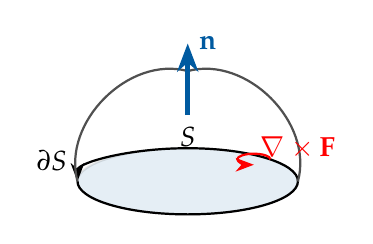
\begin{tikzpicture}[scale=0.7, >=Stealth]
    \draw[thick, fill=themeblue, opacity=0.1] (0,0) ellipse (2 and 0.6);
    \draw[thick, ->] (2,0) arc (0:180:2 and 0.6) node[above left] {$\partial S$};
    \draw[thick] (-2,0) arc (180:360:2 and 0.6);
    \draw[thick, themegray] (2,0) to [bend right=60] (0,2) to [bend right=60] (-2,0);
    \draw[->, themeblue, ultra thick] (0,1.2) -- (0,2.5) node[right] {$\mathbf{n}$};
    \node at (0,0.8) {$S$};
    \draw[->, red, thick] (1.5, 0.4) arc (0:270:0.3 and 0.1);
    \node[red] at (2,0.6) {$\nabla \times \mathbf{F}$};
\end{tikzpicture}
\end{center}

\textbf{Gauss's Divergence Theorem (3D Volume to Surface):} \\
$\iiint_V (\nabla \cdot \mathbf{F}) \, dV = \oiint_{\partial V} \mathbf{F} \cdot d\mathbf{S}$.

\cheatsheetsubsection{Applications in Physics \& Transport}
\begin{itemize}[leftmargin=*, nosep]
    \item \textbf{Leibniz Integral Rule (Reynolds Transport Theorem):} For a deforming volume $V(t)$: \\
    $\frac{d}{dt} \iiint_{V(t)} f \, dV = \iiint_{V(t)} \frac{\partial f}{\partial t} \, dV + \oiint_{\partial V(t)} f(\mathbf{v} \cdot \mathbf{n}) \, dS$.
    \item \textbf{Continuity Equation (Mass Conservation):} $\frac{\partial \rho}{\partial t} + \nabla \cdot (\rho \mathbf{v}) = 0$.
    \item \textbf{Vorticity:} $\boldsymbol{\omega} = \nabla \times \mathbf{u}$. Represents the local spin of a fluid parcel.
\end{itemize}

\textbf{Maxwell's Equations (Vacuum):}
\begin{enumerate}[label=\arabic*., leftmargin=*, nosep]
    \item Gauss's Law: $\nabla \cdot \mathbf{E} = \rho / \varepsilon_0$
    \item Gauss's Law for Magnetism: $\nabla \cdot \mathbf{B} = 0$
    \item Faraday's Law: $\nabla \times \mathbf{E} = -\frac{\partial \mathbf{B}}{\partial t}$
    \item Ampere-Maxwell Law: $\nabla \times \mathbf{B} = \mu_0 \mathbf{J} + \mu_0 \varepsilon_0 \frac{\partial \mathbf{E}}{\partial t}$
\end{enumerate}
\textbf{Derivation of Wave Equation:} $\nabla \times (\nabla \times \mathbf{E}) \implies \nabla^2 \mathbf{E} = \mu_0 \varepsilon_0 \frac{\partial^2 \mathbf{E}}{\partial t^2} = \frac{1}{c^2} \frac{\partial^2 \mathbf{E}}{\partial t^2}$.

\cheatsheetsection{9. Practical Intuition \& Workflows}

\cheatsheetsubsection{Theorem Selection Guide}
\begin{itemize}[leftmargin=*, nosep]
    \item \textbf{Green's Theorem:} Use when working with a closed curve strictly in a 2D plane. Excellent for finding enclosed areas.
    \item \textbf{Stokes' Theorem:} Use when calculating the flux of a curl ($\nabla \times \mathbf{F}$) across an open surface, OR to convert a difficult surface integral into a simpler line integral along the boundary $\partial S$.
    \item \textbf{Gauss's Theorem (Divergence):} Use when evaluating the flux ($\nabla \cdot \mathbf{F}$) across a strictly closed surface (like a sphere or box) to convert it into a volume integral.
\end{itemize}

\cheatsheetsubsection{Coordinate System Strategies}
\begin{itemize}[leftmargin=*, nosep]
    \item \textbf{Cylindrical:} Optimal for symmetries around an axis (wires, cylinders, rotating bodies). Look for the term $x^2 + y^2$.
    \item \textbf{Spherical:} Optimal for point symmetries radiating from an origin (spheres, cones). Look for the term $x^2 + y^2 + z^2$.
\end{itemize}

\cheatsheetsubsection{Recognizing Conservative Fields ($\mathbf{F}$)}
Equivalent conditions on a simply connected domain:
\begin{itemize}[leftmargin=*, nosep]
    \item \textbf{Irrotational:} $\nabla \times \mathbf{F} = \mathbf{0}$.
    \item \textbf{Scalar Potential:} $\mathbf{F} = \nabla f$.
    \item \textbf{Path Independence:} $\int_C \mathbf{F} \cdot d\mathbf{r}$ depends only on endpoints.
    \item \textbf{Zero Circulation:} $\oint_C \mathbf{F} \cdot d\mathbf{r} = 0$ for any closed loop.
\end{itemize}
In practice, if $\nabla \times \mathbf{F} = \mathbf{0}$, you can find a potential $f$ and use the Fundamental Theorem: $W = f(B) - f(A)$, completely avoiding the line integral calculation.

\cheatsheetsection{10. \textbf{CORE}: Exam Quick-Formulas}
\vspace{0.2em}
\renewcommand{\arraystretch}{1.4}

{\color{themeblue}\normalsize\bfseries A. Differential Operators \& Position Vector} \par
\vspace{-0.2em}
\begin{tabularx}{\linewidth}{|X|}
\hline
\textbf{1.} $\nabla f = \langle f_x, f_y, f_z \rangle$ (Gradient: normal to level curves. Max directional derivative $D_{\mathbf{u}}f = |\nabla f|$) \\
\textbf{2.} $\nabla \cdot \mathbf{F} = P_x + Q_y + R_z$ (Divergence: source/sink flux density at a point) \\
\textbf{3.} $\nabla \times \mathbf{F} = \langle R_y-Q_z, P_z-R_x, Q_x-P_y \rangle$ (Curl: axis and magnitude of local rotation) \\
\textbf{4.} $\nabla^2 f = \nabla \cdot \nabla f = f_{xx} + f_{yy} + f_{zz}$ (Laplacian: concavity/diffusion of a scalar field) \\
\textbf{5.} Position Vector $\mathbf{r} = \langle x, y, z \rangle$ with magnitude $r = |\mathbf{r}| = \sqrt{x^2+y^2+z^2}$ \\
\textbf{6.} $\nabla \cdot \mathbf{r} = 3 \quad \text{and} \quad \nabla \times \mathbf{r} = \mathbf{0}$ (Radial fields are irrotational) \\
\textbf{7.} $\nabla (r^n) = n r^{n-2} \mathbf{r} \implies \nabla(r) = \hat{r}, \quad \nabla\left(\frac{1}{r}\right) = -\frac{\mathbf{r}}{r^3}, \quad \nabla^2\left(\frac{1}{r}\right) = 0 \text{ } (r \neq 0)$ \\
\hline
\end{tabularx}

\vspace{0.6em}
{\color{themeblue}\normalsize\bfseries B. Key Vector Identities} \par
\vspace{-0.2em}
\begin{tabularx}{\linewidth}{|X|}
\hline
\textbf{8.} $\nabla \times (\nabla f) = \mathbf{0}$ (The curl of a gradient is strictly zero) \\
\textbf{9.} $\nabla \cdot (\nabla \times \mathbf{F}) = 0$ (The divergence of a curl is strictly zero) \\
\textbf{10.} $\nabla \times (\nabla \times \mathbf{F}) = \nabla(\nabla \cdot \mathbf{F}) - \nabla^2\mathbf{F}$ (Double curl identity) \\
\textbf{11.} $\nabla \cdot (\phi \mathbf{F}) = \phi(\nabla \cdot \mathbf{F}) + \mathbf{F} \cdot (\nabla \phi)$ (Divergence product rule) \\
\textbf{12.} $\nabla \times (\phi \mathbf{F}) = \phi(\nabla \times \mathbf{F}) + (\nabla \phi) \times \mathbf{F}$ (Curl product rule) \\
\textbf{13.} $\nabla \cdot (\mathbf{A} \times \mathbf{B}) = \mathbf{B} \cdot (\nabla \times \mathbf{A}) - \mathbf{A} \cdot (\nabla \times \mathbf{B})$ \\
\hline
\end{tabularx}

\newpage
{\color{themeblue}\normalsize\bfseries C. Fundamental Integral Theorems} \par
\vspace{-0.2em}
\begin{tabularx}{\linewidth}{|X|}
\hline
\textbf{14.} $W = \int_C \mathbf{F} \cdot d\mathbf{r} = \int_a^b \mathbf{F}(\mathbf{r}(t)) \cdot \mathbf{r}'(t) dt$ (Work or Circulation) \\
\textbf{15.} $\Phi = \iint_S \mathbf{F} \cdot \mathbf{n} \, dS$ (Surface Flux) \\
\textbf{16.} $\mathbf{F} = \nabla f \implies \int_A^B \mathbf{F} \cdot d\mathbf{r} = f(B) - f(A)$ (Fund. Theorem of Line Integrals) \\
\textbf{17.} $\oint_C (P dx + Q dy) = \iint_D (Q_x - P_y) dA$ (Green's Theorem - Circulation Form) \\
\textbf{18.} $\oint_C (-Q dx + P dy) = \iint_D (P_x + Q_y) dA$ (Green's Theorem - Flux Form 2D) \\
\textbf{19.} $\oint_{\partial S} \mathbf{F} \cdot d\mathbf{r} = \iint_S (\nabla \times \mathbf{F}) \cdot d\mathbf{S}$ (Stokes' Theorem: boundary to surface) \\
\textbf{20.} $\oiint_{\partial V} \mathbf{F} \cdot d\mathbf{S} = \iiint_V (\nabla \cdot \mathbf{F}) dV$ (Gauss's Theorem: closed surface to volume) \\
\textbf{21.} $\iiint_V (\phi\nabla^2\psi + \nabla\phi\cdot\nabla\psi)dV = \oiint_{\partial V} \phi(\nabla\psi\cdot\mathbf{n})dS$ (Green's First Identity) \\
\textbf{22.} $\iiint_V (\phi\nabla^2\psi - \psi\nabla^2\phi)dV = \oiint_{\partial V} (\phi\nabla\psi - \psi\nabla\phi)\cdot\mathbf{n} dS$ (Green's Second Identity) \\
\textbf{23.} $Area = \frac{1}{2} \oint_C (x dy - y dx) = \oint_C x dy = -\oint_C y dx$ (Area via Green's Theorem) \\
\hline
\end{tabularx}

\vspace{0.6em}
{\color{themeblue}\normalsize\bfseries D. Time-Savers: Differentials \& Jacobians} \par
\vspace{-0.2em}
\begin{tabularx}{\linewidth}{|X|}
\hline
\textbf{24. Sphere (rad. $a$):} $d\mathbf{S} = \hat{r} \, a^2 \sin\phi \, d\phi \, d\theta$. Jacobian $|J| = r^2\sin\phi$ \\
\textbf{25. Cylinder (rad. $a$):} $d\mathbf{S} = \hat{\rho} \, a \, dz \, d\theta$. Jacobian $|J| = \rho$ \\
\textbf{26. Graph $z = f(x,y)$:} $d\mathbf{S} = \pm \langle -f_x, -f_y, 1 \rangle dA \implies dS = \sqrt{f_x^2 + f_y^2 + 1} \, dA$ \\
\textbf{27. Normal Line to $F=k$:} $\mathbf{r}(t) = \mathbf{r}_0 + t\nabla F(\mathbf{r}_0)$ \\
\hline
\end{tabularx}

\vspace{0.6em}
{\color{themeblue}\normalsize\bfseries E. Common Pitfalls \& Quick Checks} \par
\vspace{-0.2em}
\begin{tabularx}{\linewidth}{|X|}
\hline
\textbf{28. Stokes' Orientation (RHR):} If walking along $\partial S$ with head aligned with normal $\mathbf{n}$, surface $S$ must be on your left. \\
\textbf{29. Conservative Field:} $\mathbf{F} = \nabla \phi \iff \nabla \times \mathbf{F} = \mathbf{0}$ (Irrotational). \\
\textbf{30. Vector Potential:} $\mathbf{F} = \nabla \times \mathbf{A} \iff \nabla \cdot \mathbf{F} = 0$ (Solenoidal). \textit{Tip: Use Stokes to find flux of a solenoidal field over open surfaces!} \\
\hline
\end{tabularx}

\end{document}